\section{Results}
In this section, the results are presented using tables and charts. Note that on some charts the vertical axis is base 10 logarithmic (for viewing purposes). The implementation of all the algorithms for all languages can be found in Appendix \ref{appendix:code}.

\subsection{Native environments}
This section display the results for the tests made in each language native environment. As is illustrated in each subsection, these tests tend to do better performance wise than the corresponding tests in the .NET environment.

\subsubsection{Addition Operator}

The test takes 10 million positive randomly generated integers and calculates the sum of them. See Figure \ref{fig:native_addition} for results. Other operators such as subtraction, multiplication, division and modulo were also tested but generated the same results except in the case of Python where they were all slower due to the sum function being more efficient than the reduce function.

\begin{figure}[h]
	\centering
	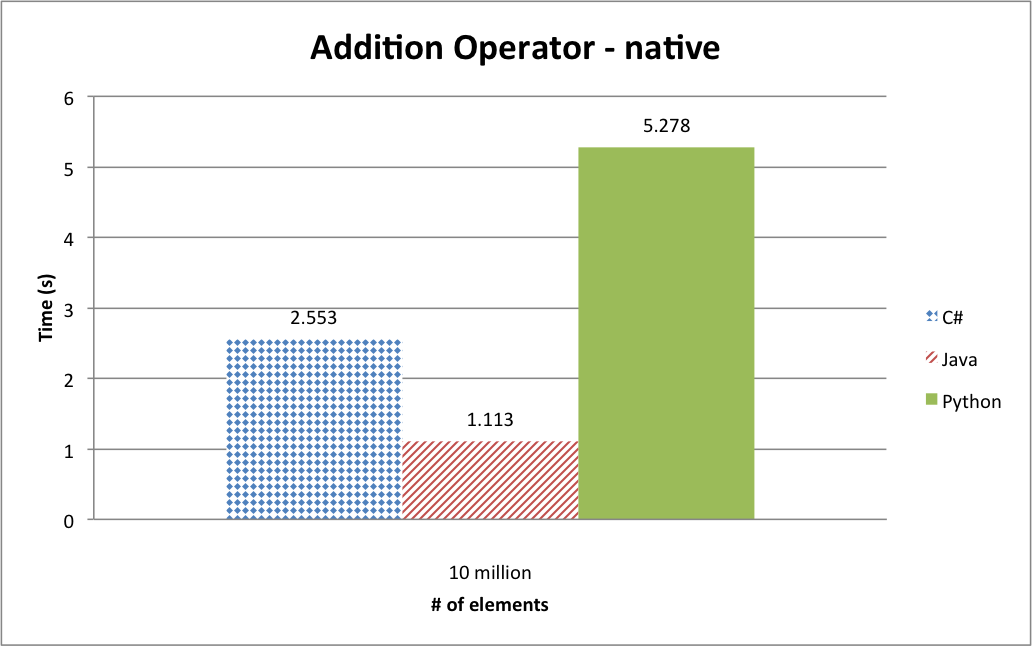
\includegraphics[width=1.0\linewidth]{chapters/new_media/AdditionOperatorNative.png}
	\caption{This tests a language ability to sum 10 million elements. Lower is better. The results show that Java running in its native environment is the fastest of the three languages with 1.113 seconds. Python is the slowest of the three with a runtime of 5.278 seconds, even when using its native library functions to sum the elements, see \ref{appendix:code_addition}.}
	\label{fig:native_addition}
\end{figure}


\subsubsection{Insertion Sort}

Figure \ref{fig:native_insertion_sort} illustrates the time it takes for each language to sort 10'000 randomly generated positive integers in ascending order. Note the severe time differences between Python and the other languages.

\begin{figure}[h]
	\centering
	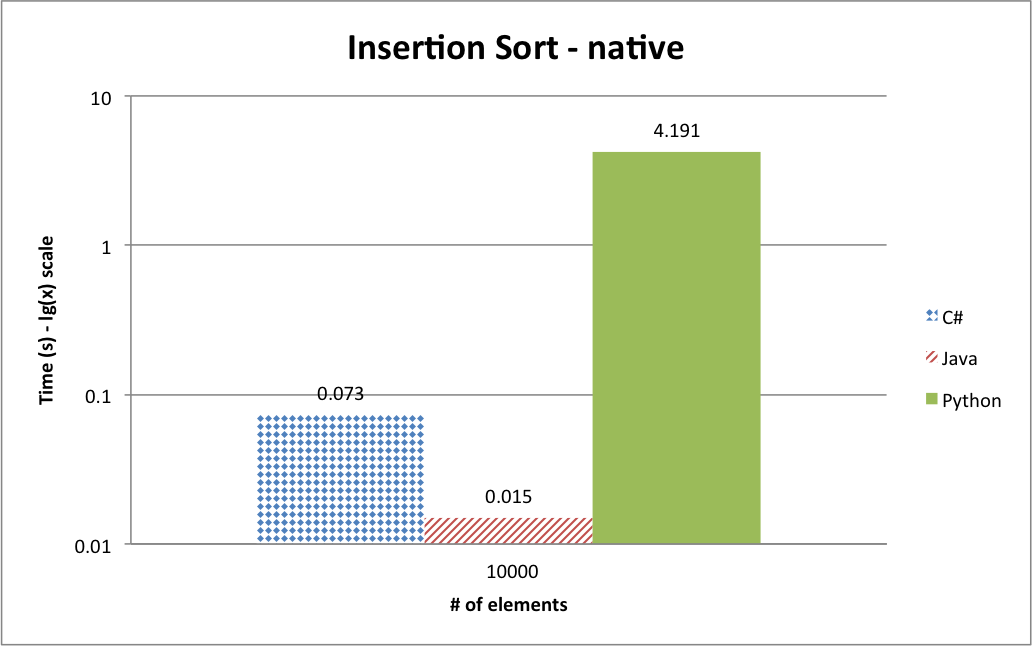
\includegraphics[width=1.0\linewidth]{chapters/new_media/InsertionSortNative.png}
	\caption{This test uses the Insertionsort algorithm to sort 10'000 elements in ascending order. Lower is better. Please note that the vertical axis is base 10 logarithmic. Java is the fastest with 0.015 seconds while Python is the slowest with 4.191 seconds. }
	\label{fig:native_insertion_sort}
\end{figure}


\subsubsection{Merge Sort}

Figure \ref{fig:native_merge_sort} illustrates the time it takes for each language to sort one million randomly generated positive integers in ascending order.

\begin{figure}[h]
	\centering
	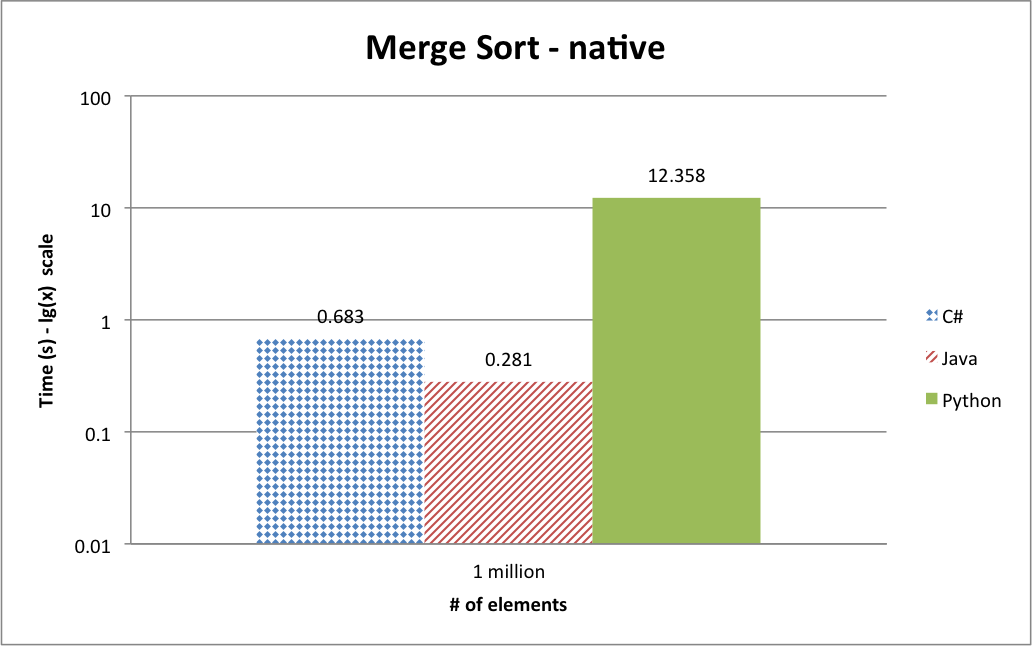
\includegraphics[width=1.0\linewidth]{chapters/new_media/MergeSortNative.png}
	\caption{This test uses the Merge sort algorithm to sort one million elements in ascending order. Lower is better. Note that the vertical axis is base 10 logarithmic. Java is the fastest with 0.281 seconds while Python is the slowest with 12.358 seconds.}
	\label{fig:native_merge_sort}
\end{figure}


\subsection{.NET environment}
This section display the results for the tests made in each language when run in the .NET environment. The tests tend to perform poorer performance wise than the corresponding tests in the native environment.

\subsubsection{Language Overhead} \label{subsec:language_overhead}

\begin{table}[h]
	\begin{center}
		\begin{tabular} { >{\centering\arraybackslash}m{3cm} | >{\centering\arraybackslash}m{2cm}}
			\hline
			\textbf{Language}	& \textbf{Time} \\ \hline
			C\#					& 0.014s \\ \hline
			Java				& 0.038s \\ \hline
			Python				& 1.006s \\ \hline
		\end{tabular}
	\end{center}
	\caption{The overhead startup cost for each language when run in the .NET environment. Since C\# is the native language it has the lowest startup time with 0.014 seconds while Python has the longest with 1.006 seconds.}
	\label{table:language_overhead}
\end{table}

As can be seen in Table \ref{table:language_overhead} Python has a greater overhead cost than the other two.


\subsubsection{Addition Operator}

The test takes 10 million positive randomly generated integers and calculates the sum of them. See Figure \ref{fig:net_addition} for results. Other operators such as subtraction, multiplication, division and modulo were also tested but generated the same results except in the case of Python where they were all slower due to the sum function being more efficient than the reduce function.

\begin{figure}[h]
	\centering
	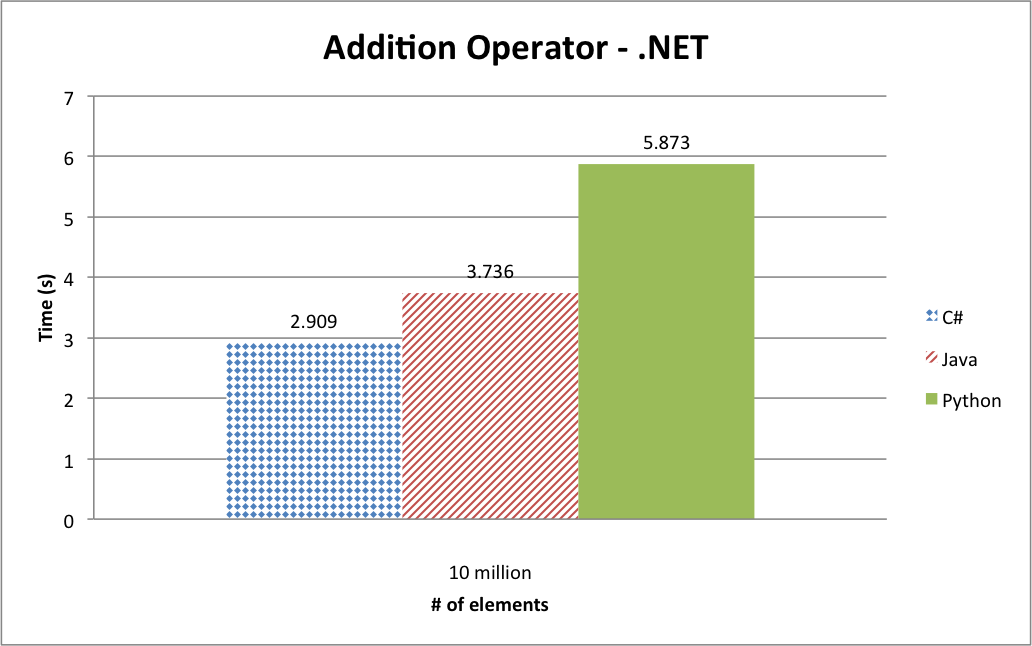
\includegraphics[width=0.7\linewidth]{chapters/new_media/AdditionOperatorNet.png}
	\caption{This tests a language ability to sum 10 million elements. Lower is better. The results show that C\# running in its native environment (.NET) was the fastest of the three languages with 2.909 seconds. Python was the slowest of the three with a runtime of 4.867 seconds.}
	\label{fig:net_addition}
\end{figure}


\subsubsection{Insertion Sort}

Figure \ref{fig:net_insertion_sort} illustrates the time it takes for each language, run in the .NET environment, to sort 10'000 randomly generated positive integers in ascending order.

\begin{figure}[h]
	\centering
	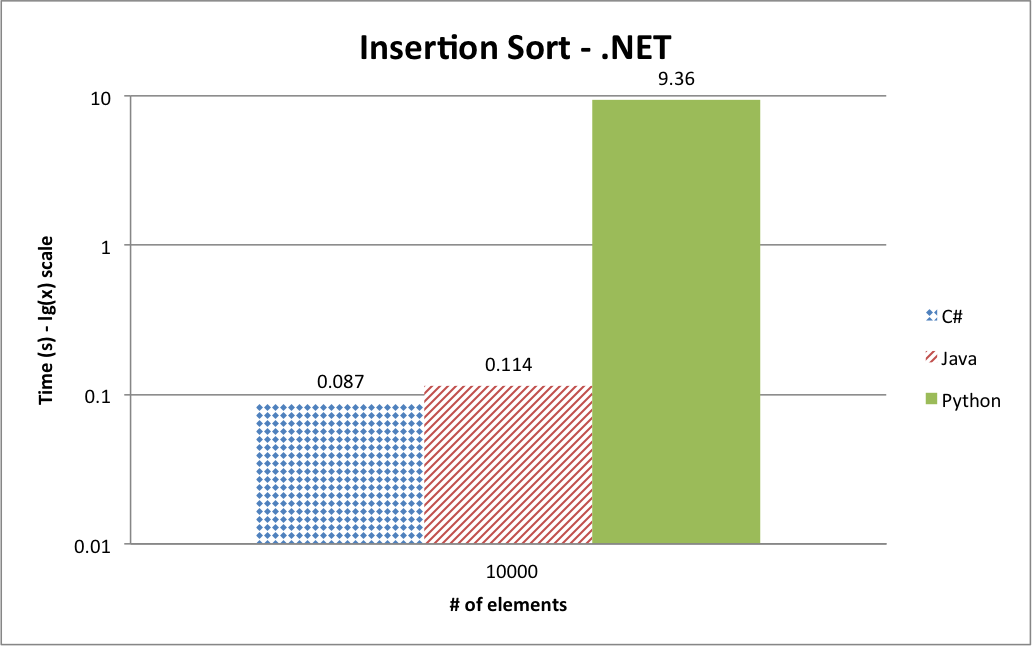
\includegraphics[width=0.7\linewidth]{chapters/new_media/InsertionSortNet.png}
	\caption{This test was run in the .NET environment and used the Insertion sort algorithm to sort 10'000 elements in ascending order. Lower is better. Note that the vertical axis is base 10 logarithmic. C\# was the fastest with 0.087 seconds. Java was a close second with 0.114 seconds. Python was the worst with 9.36 seconds.}
	\label{fig:net_insertion_sort}
\end{figure}


\subsubsection{Merge Sort}

Figure \ref{fig:net_merge_sort} illustrates the time it takes for each language, run in the .NET environment, to sort one million randomly generated positive integers in ascending order.

\begin{figure}[h]
	\centering
	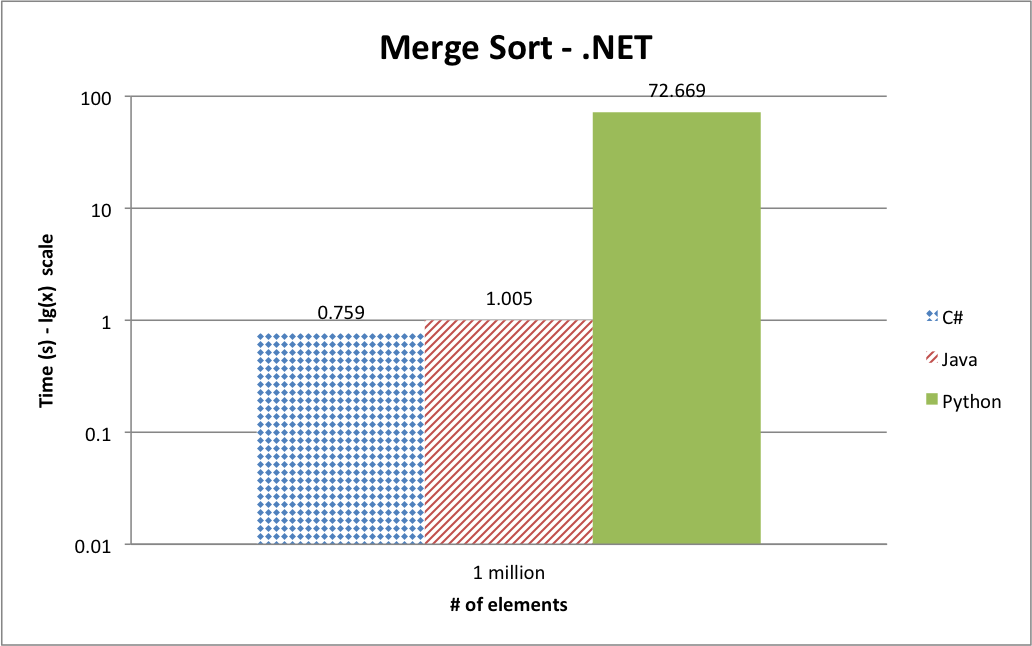
\includegraphics[width=1.0\linewidth]{chapters/new_media/MergeSortNet.png}
	\caption{This test was run in the .NET environment and used the Merge sort algorithm to sort one million elements in ascending order. A lower value is better. Note that the vertical axis is base 10 logarithmic. C\# was the fastest with 0.759 seconds. Java came in second with 0.967 seconds. Python was the slowest with 71.663 seconds.}
	\label{fig:net_merge_sort}
\end{figure}

Figure \ref{fig:net_merge_sort_memory} illustrates the amount of MB of memory used when running the merge sort algorithm in the .NET environment by the different languages. C\# and Java are almost equal while Python uses more memory.

\begin{figure}[h]
	\centering
	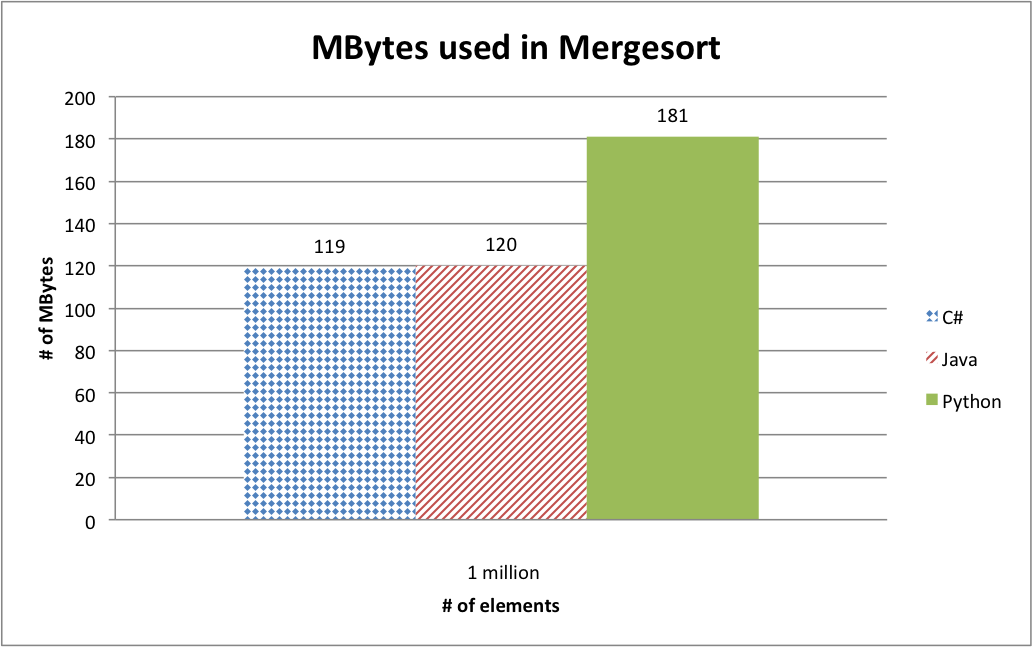
\includegraphics[width=1.0\linewidth]{chapters/new_media/MBytesMergesort.png}
	\caption{This test was run in the .NET environment and used the Merge sort algorithm to sort one million elements in ascending order. A lower value is better. C\# and Java performed almost equally with 119MB and 120MB of memory used. Python performed the worst with 181MB of memory used. }
	\label{fig:net_merge_sort_memory}
\end{figure}


